\subsection{Что мы хотим от системы}

В рамках курсового проекта рассматривается система управления и оркестрации заказов,
которая должна помочь организовать устойчивую и понятную работу с потоком заявок
в условиях роста нагрузки. Функционал система это не только обработка заказов,
но и их полный жизненный цикл.

Ключевые задачи, которые должна решать целевая система:
\begin{itemize}
  \item централизованное управление заказами в рамках одной системы;
  \item предсказуемая обработка заказов и снижение накладных расходов;
  \item прозрачность этапов обработки заказов;
  \item масштабируемость процессов при росте системы.
\end{itemize}

Далее рассмотрены рыночные аналоги с точки зрения того, насколько полно
они закрывают перечисленные потребности.

\subsection{Аналог 1: Odoo}

Odoo является модульной ERP-платформой, которая часто применяется для автоматизации продаж, учета и 
иных связанных процессов. Решение ориентировано на комплексное ведение бизнеса
в единой системе и позволяет достаточно быстро запустить базовые процессы.

Иллюстрация интерфейса решения приведена на рисунке~\ref{fig:odoo_ui}.

\begin{figure}[htbp]
  \centering
  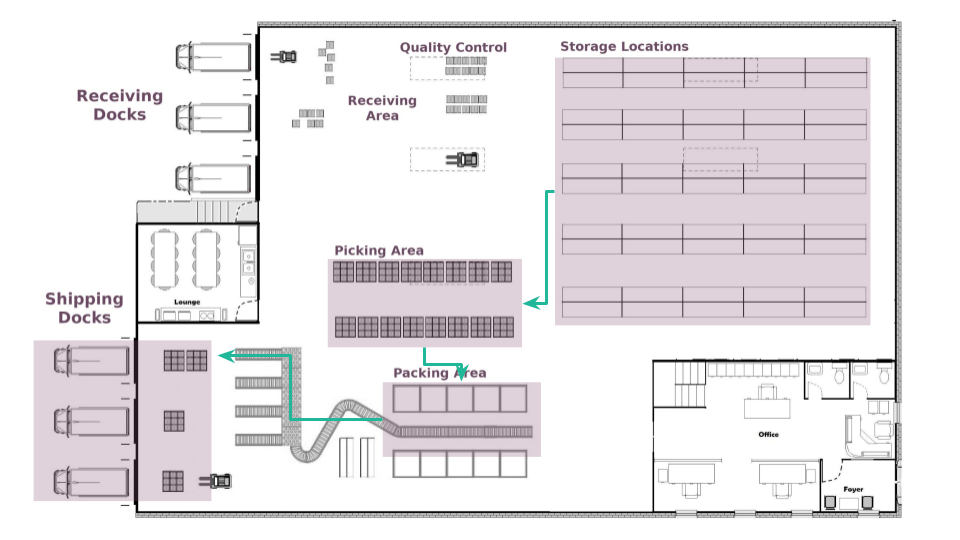
\includegraphics[width=0.95\textwidth]{images/odoo.png}
  \caption{Пример интерфейса Odoo для работы с заказами}
  \label{fig:odoo_ui}
\end{figure}

Сильные стороны Odoo в контексте поставленной задачи:
\begin{itemize}
  \item единая среда для работы с заказами и складскими операциями;
  \item относительно быстрый старт для типовых сценариев;

\end{itemize}

Ограничения Odoo в контексте проекта:
\begin{itemize}
  \item для узкоспециализированной оркестрации заказов требуется заметная доработка;
  \item часть бизнес-правил удобнее реализуется через кастомизацию, что усложняет поддержку;
  \item при усложнении процессов возрастает зависимость от конкретной конфигурации системы.
\end{itemize}

Odoo демонстрирует ценность единого операционного контура и удобства
ежедневной работы, что следует учитывать как ориентир для собственной системы.
При этом для рассматриваемой предметной области важно заранее учитывать, что
по мере роста объема операций потребуется более строгая регламентация внутренних
процессов, чем это предусмотрено в типовой конфигурации.

\subsection{Аналог 2: SAP Extended Warehouse Management}

SAP EWM используется преимущественно на крупных предприятиях и ориентирована
на зрелые складские и логистические процессы. Система покрывает широкий круг
задач управления операциями и хорошо подходит разным организациям.

Пример интерфейса SAP EWM показан на рисунке~\ref{fig:sap_ui}.

\begin{figure}[htbp]
  \centering
  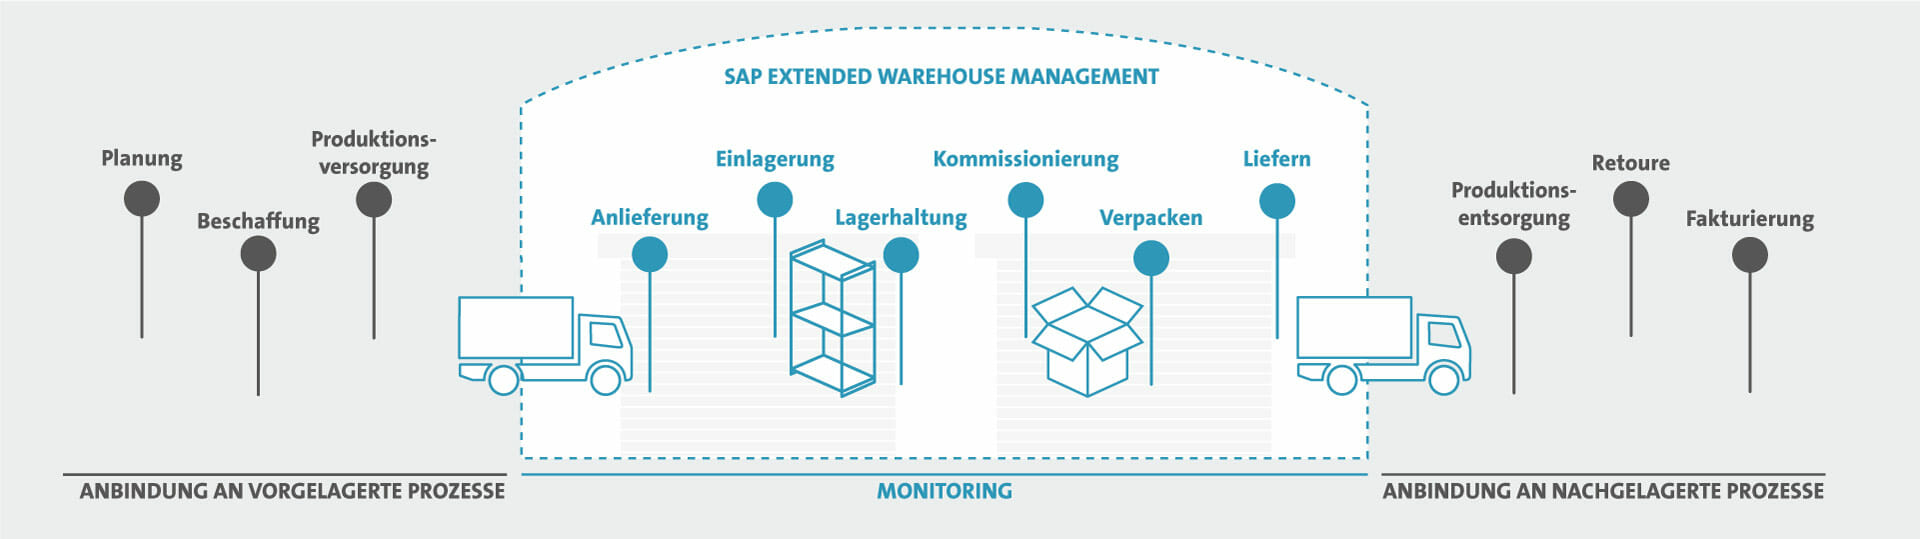
\includegraphics[width=0.95\textwidth]{images/sap.jpg}
  \caption{Пример рабочего экрана SAP Extended Warehouse Management}
  \label{fig:sap_ui}
\end{figure}

Сильные стороны SAP EWM в контексте потребностей:
\begin{itemize}
  \item высокая процессная дисциплина и детальная проработка операций;
  \item хорошая управляемость больших объемов заказов;
  \item высокая прозрачность состояния операций в рамках компании.
\end{itemize}

Ограничения SAP EWM в контексте проекта:
\begin{itemize}
  \item высокая стоимость внедрения и сопровождения;
  \item длительный цикл внедрения и адаптации под конкретную организацию;
\end{itemize}

SAP EWM задает ориентир по масштабу и управляемости процессов,
но по сложности и стоимости не соответствует формату курсового проекта.
Для целей текущей разработки этот аналог полезен прежде всего как референс
по глубине процессной декомпозиции и по уровню прозрачности исполнения операций.

\subsection{Аналог 3: Oracle Warehouse Management}

Oracle Warehouse Management является корпоративным решением для управления
складскими и смежными операциями в организациях. Продукт ориентирован
на стабильную работу и унификацию процессов.

Пример интерфейса Oracle Warehouse Management приведен на рисунке~\ref{fig:oracle_ui}.

\begin{figure}[htbp]
  \centering
  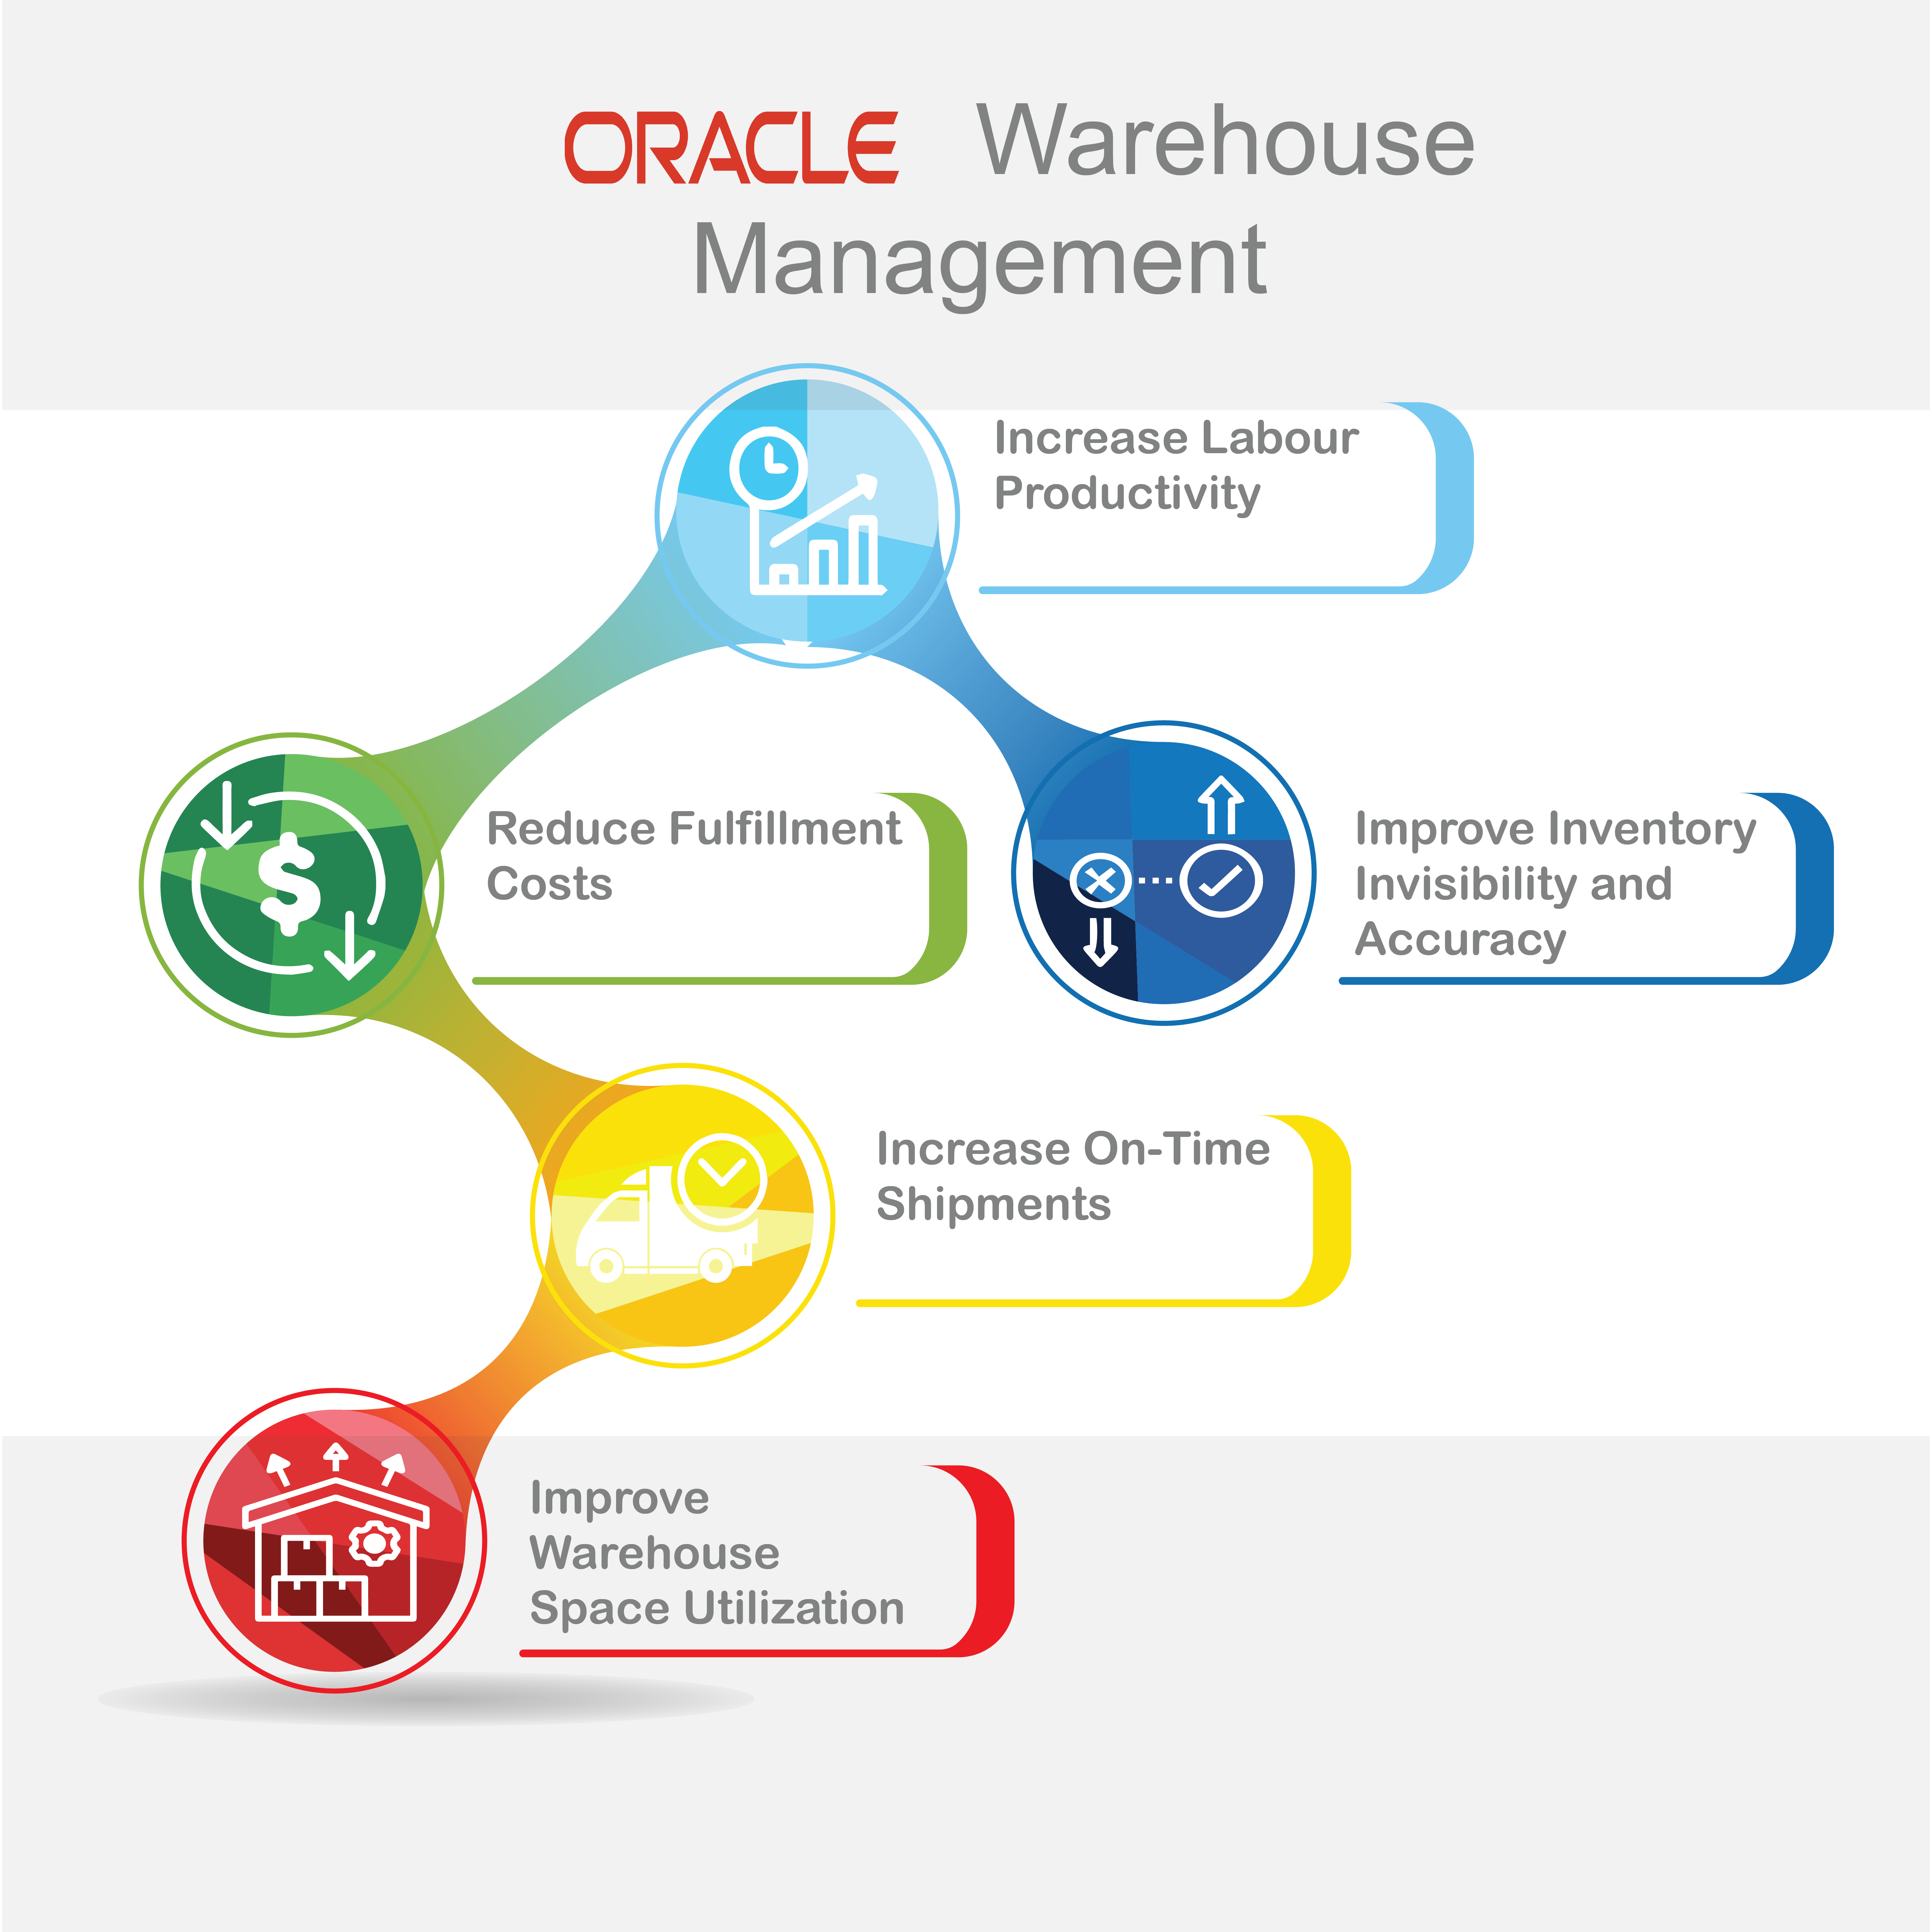
\includegraphics[width=0.95\textwidth]{images/oracle.png}
  \caption{Пример интерфейса Oracle Warehouse Management}
  \label{fig:oracle_ui}
\end{figure}

Сильные стороны Oracle Warehouse Management:
\begin{itemize}
  \item развитые средства контроля операционных этапов;
  \item возможность работы с большими потоками заказов;
  \item интеграция в корпоративную экосистему управления ресурсами.
\end{itemize}

Ограничения Oracle Warehouse Management:
\begin{itemize}
  \item высокий порог входа и значительные организационные затраты на внедрение;
  \item невысокая гибкость для быстрого изменения узкоспециализированных сценариев;
\end{itemize}

Oracle Warehouse Management  не является оптимальной основой для компактного и гибкого решения
в рамках текущего проекта.
Тем не менее анализ данного продукта подтверждает практическую значимость
централизованного контроля этапов обработки заказов в условиях высокой нагрузки.

\subsection{Итоговый вывод по анализу аналогов}

Проведенный анализ показывает, что рыночные продукты закрывают значительную часть
потребностей по управлению заказами и прозрачности операций, но делают это в разных
приоритетах: одни лучше подходят для быстрого старта и базовой автоматизации,
другие ориентированы на крупный масштаб и строго регламентированные процессы.

В рамках курсового проекта будет сспроектирована собственная
система, в которой фокус будет сделан на целевые потребности: централизованное
управление заказами, отказоустойчивость обработки,
прозрачность этапов и масштабируемость по объему операций.

Таким образом, анализ аналогов подтверждает, что выбранная тема проекта
практически обоснована: в существующих продуктах есть полезные подходы,
но в рамках учебной задачи и заданного контекста требуется более компактное,
предметно-ориентированное и управляемое по сложности решение.
